%*****************************************
\chapter{Theory and Alternatives}\label{ch:theory_and_alternatives}
%*****************************************

\section{Category Learning}

\begin{equation}
({\forall}x~{\in}~X)[(h_k(x)=1){\rightarrow}(h_j(x)=1)]
\end{equation}

\section{Two Popular Approaches to Modelling Intelligence}

Recently, there have been two directions of research with the goal of
building a machine that explains intelligent human behavior.  The
first approach is to build a baby-machine that learns from scratch to
accomplish goals through interactions with its environment.  The
second approach is to give the machine an abundance of knowledge that
represents correct behavior.

Each of these solutions has benefits and drawbacks.  The baby-machine
approach is good for dealing with novel problems, but these problems
are necessarily simple because complex problems require a lot of
background knowledge.  The data abundance approach deals well with
complicated problems requiring a lot of background knowledge, but
fails to adapt to changing environments, for which the algorithm has
not already been trained.

\subsection{Adaptability in Complex Environments}

\begin{figure}[bth]
  \center
  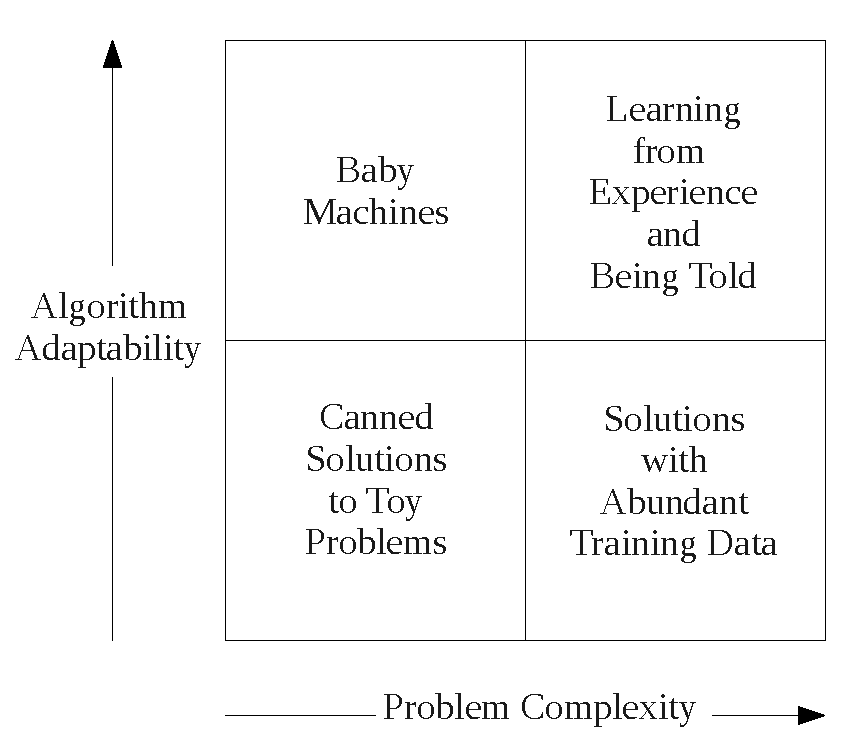
\includegraphics[height=6cm]{gfx/problem_complexity_versus_algorithm_adaptability}
  \caption[Problem complexity versus algorithm adaptability]{Problem
    complexity versus algorithm adaptability.}
  \label{fig:problem_complexity_versus_algorithm_adaptability}
\end{figure}

We would like to build intelligent machines that are able to perform
household tasks, such as cooking, cleaning, and doing the laundry, but
these tasks seem insurmountably complex, containing organically
unpredictable events.  We would like our machines to expertly handle
these extremely complicated problems, and we would also like them to
adapt to learn in unexpected or novel situations.  One popular
approach to building a machine that performs complicated tasks is to
give the machine a large training dataset that details every possible
situation that the machine may find itself within, along with the
correct action in that situation.  This is the so-called
``supervised'' learning approach.  These algorithms do not adapt to
novel situations well, and collecting these datasets is often
impossible for many problems, such as cooking and cleaning because it
is too difficult to enumerate all possible situations, in which the
machine may find itself.  Also, if the machine is cooking a meal, we
would like to be able to explain an idea for a new recipe to the
machine, or to perhaps be a partner in discovering new recipes, or we
may simply want to explain to the machine that a guest has a specific
allergy to walnuts, making that ingredient an exception for this meal
but not others.
Figure~\ref{fig:problem_complexity_versus_algorithm_adaptability}
shows how problem complexity and algorithm adaptability can be thought
of as a two-dimensional space into which different algorithmic
approaches can be used as solutions.

\subsection{The Abundant Data Approach}

There have been many approaches to modelling complex forms of
reasoning by collecting large amounts of knowledge that describes
correct or acceptable behavior in a domain.  For example, there are
examples of complex multi-AI commonsense simulation environments
collects thousands of examples of users interacting in a complicated
object-oriented social simulation \citep{orkin:2009},
\citep{orkin:2010}.  These systems have complicated domains, but these
projects do not attempt to build AIs that attempt to accomplish
goals.  Instead, these systems are inference systems that simply try
to reproduce typical behavior, rather than goal-directed behavior.

There are many commonsense reasoning systems that do not interact with
simulation environments at all, but which attempt to demonstrate
commonsense reasoning by being told large amounts of knowledge.  The
Cyc project is one large such project that has been told large amounts
of logical knowledge \citep{lenat:1990}.  There is also effort
directed toward populating Cyc with knowledge automatically gathered
from the web \citep{matuszek:2005}.  The OpenMind project
\citep{singh:2002} is a project that gathers large amounts of
approximately correct commonsense knowledge from people online.  The
OpenMind knowledge has been turned into many inference systems that
can compare and generate new commonsense knowledge \citep{liu:2004a,
  liu:2004b, speer:2009}.

\subsection{The Common Sense Reasoning Problem Domain}

Common sense is the set of common reasoning abilities shared by most
people in a given social group.  Another way to say this is that
common sense is the set of reasoning abilities that one would assume
of a typical person that they meet for the first time and know nothing
about.  For example, most people have a naive theory of physics, so
you would expect someone to know that things fall when they are not
supported and liquids flow or are absorbed unless they are in a
container.  Common sense relies on a lot of knowledge that is assumed
that most everyone knows.

%TS>> what is a given social group... i share very little reasoning abiltities about user TS>>interface with my daughter or the director of CMU Siliicon Valley or my bike riding 
%TS>> friends, or my brothers,....

%TS>> not crisp enough ... a person is not defined as a person...but realtive to a 
%TS>> role we have with them,,, a mechanic talks differently to a woman or man, a professor
%TS>> or his accountant about cars 

%TS>> again, people have different theories of physics than each other 

%TS>> i have been served food in which the floating stuff  was designed to change through 
%TS>> the period of servign and eating soup  ..

%TS>> I am ready for  a fight on that , i live with a woman, a teenage girl, an autistic,
%TS>> my neighbor is a morman, the woman next door is totally rich... very diffferent 
%TS>> world views... even about how to deal with trash from a dinner. 

%TS>> I don't know what YOU mean by common sense yet,,,, define something specific
%TS>> does it cover diffferent minds or clones, what about its edges,   


Building a machine that demonstrates common sense reasoning is a
long-standing goal of the field of artificial intelligence.  One of
the difficulties in developing algorithms for dealing with a common
sense reasoning domain is that the algorithm needs a lot of background
knowledge about a given domain before it can answer even simple
questions about it.  However, this knowledge is often only true in
very specific situations and has many exceptional cases.  For example,
the knowledge that most birds can fly is generally true, but we also
know that many birds are flightless, such as penguins, ostriches, and
road runners.  Also, we have knowledge about the typical behavior of
objects; for example, we know that refrigerators keep things cold,
but we also reason efficiently about exceptional cases, such as when
the refrigerator is not plugged in, or when the power goes out.

%TS>> yes but those are examples we have seen for decades with varying 
%TS>> logical relations solving them
%TS>> show some that we haven't been able to do or places where you hold
%TS>> up where others have always been brittle 
%TS>> flexibility, integrity, hypocracy, intentionality changing belief systems...? 


\subsection{Representations for Common Sense Reasoning}

There have been many approaches to artificial intelligence that use
first-order logic as a representation for these types of knowledge and
their exceptions, but these systems become cumbersome in their
inability to express ``fuzzy'' sorts of relationships, such as when
the knowledge is applicable, for example the modifiers, ``most of the
time'', ``usually'', and ``almost never'', are difficult to express in
first-order logic.  When we have a lot of knowledge, we need ways to
keep track of in which situations this knowledge is useful.  This is a
form of ``meta-knowledge'', or knowledge about knowledge.
Meta-knowledge about first-order logic cannot be expressed in
first-order logic, so another type of representation is required for
this type of knowledge.  Therefore, we need other ways to represent
our knowledge in addition to logic.

\begin{quote}
``Nonetheless, theorem proving is in the worst case an intractable
  problem, even with no variables or unification, so no algorithm is
  going to work on the problem all the time. In this respect, theorem
  proving, for all its superficial formalism, is a lot like other
  branches of AI.  Where a theorist views a problem as solved if he
  has found an efficient algorithm or a discouraging lower bound, an
  AI researcher is often happy to find an algorithm that seems to work
  on some interesting problems, even though he doesn't really know the
  bounds of what it can do. Exploration will reveal the extent of its
  powers-each time it solves one more interesting problem something
  has been
  gained.''~---~\defcitealias{mcdermott:1987}{Drew~McDermott}\citetalias{mcdermott:1987}
\end{quote}


\section{Comparable Cognitive Architectures}

EM-ONE, Cyc, Icarus, ACT-r, Soar, and Prodigy are comparable cognitive
architectures to the one that I have built.

\subsection{The EM-ONE Cognitive Architecture}

I worked with Pushpinder Singh from 1999 to 2006 on the first version
of the Emotion Machine architecture, EM-ONE \citep{singh:2005}.
EM-ONE was an example of a reflective control system that used
commonsense stories in order to reason about social problem solving.
\cite{morgan:2009} discusses a number of things to learn from the
EM-ONE architecture that have informed my current approach.

Push and I have discussed that one weakness in the EM-ONE system is
its reliance on tracing only the declarative prolog statements, among
other necessary but untraced procedural code.  Although EM-ONE
contained a large amount of procedural knowledge, none of the effects
of this procedural knowledge could be debugged reflectively.  Toward
solving this problem, I have based my approach on a memory layer that
can trace the provenance of select memory events.

\subsection{Icarus}

Icarus is a cognitive architecture that supports a form of far
transfer learning \citep{konik:2009}.  The Icarus system allows for a
goal-directed structure mapping learning process.  These structure
mappings that are learned in this goal-directed way, can be useful
forms of analogy that enables ``far'' transfer in a cognitive system.
The Icarus work builds upon a previous model for analogical transfer
learning between symbolic relational structures \citep{gentner:1983}.

Because my knowledge representation is relational and symbolic, I see
Icarus' approaches to far transfer learning as highly compatible with
my architecture's ability to support multiple knowledge domains for a
single goal-oriented problem solving AI.  I am also interested in a
technique of using differences of differences \citep{winston:1970} as
an alternative to the structure mapping form of analogical transfer.

The Icarus system has also been applied to moral reasoning tasks in
order to build a theory of moral reasoning in humans \citep{iba:2011}.
I see similar applications of my architecture to these social
reasoning domains, but my planned approach to this domain is based on
two more layers of reflective control than I have currently
implemented \citep{morgan:2011}.

\subsection{Computational Models of Cognition about Cognition}

\cite{cox:2005} gives a good overview of the cognitive sciences that
deal with the problem of thinking about thinking, or
metacognition.

\subsection{Shades of Belief as Debugging Meta-Knowledge}

\cite{stein:1995} applies a prototype system to perform reflective
case-based reasoning over shades of beliefs in knowledge.

\section{Bounded Rationality}

There is an approach of economics and game theory that is called
bounded rationality \citep{simon:1972}.  These models deal with the
time constraints of not only acting efficiently in a domain but also
in optimizing the planning actions involved in accomplishing goals.
This approach assumes that there is an absolute numerical reward value
for accomplishing goals.  In the sense that absolute values for all of
the goals of a system are seldom known in practice, the bounded
rationality approach is limited in a general sense similar to the
simpler reinforcement learning approach.

\subsection{Feedback Control Model for Accomplishing a Single Goal}

\begin{figure}[bth]
  \center
  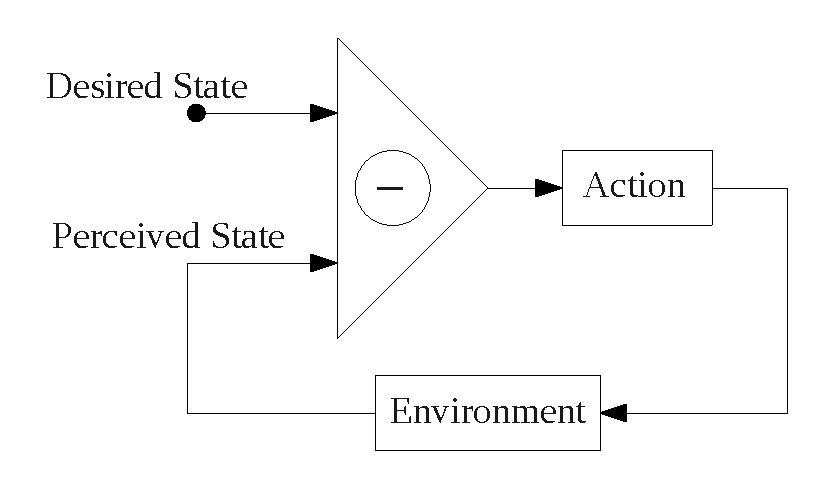
\includegraphics[width=6cm]{gfx/feedback_control}
  \caption[The feedback control model for accomplishing a single goal]{The feedback control model for accomplishing a single goal.}
  \label{fig:feedback_control}
\end{figure}

Now that we have discussed the basic model of learning from experience
what good goal states may be from rewards, let us consider the
representations for the state space of the perceptions and actions of
my model.  Control theory has given us many useful models for AIs
that control continuous environments.  For example,
Figure~\ref{fig:feedback_control} shows a simple difference feedback
control circuit that is used in simple linear control systems.  The
system is given a desired state, there is a difference device that
calculates the difference between the actual perceived value from the
environment, and the control system then executes an action based on
that difference, which affects the environment.  The result in such a
negative feedback loop is that the AI's perception of the
environment is closer to the desired state.

\subsection{Means-End Analysis}

In 1959, Newell, Shaw, and Simon published a report on a means-end
analysis model that was designed to solve any symbolically represented
problem \citep{newell:1959}.  Their system was called the \ac{GPS},
and worked by being able to work with relational representations of
current and desired states.  The AI had a catalogue of differences
between states that it knew how to minimize.  The system worked by
finding the largest difference and executing the associated method for
reducing this difference.  This work has grown into the Soar model
\citep{newell:1990} for better solving symbolic planning problems, and
dealing with impasses for when the planning search runs out of
options.

\subsection{Difference-Engine Model for Accomplishing Multiple Goals}

\begin{figure}[bth]
  \center
  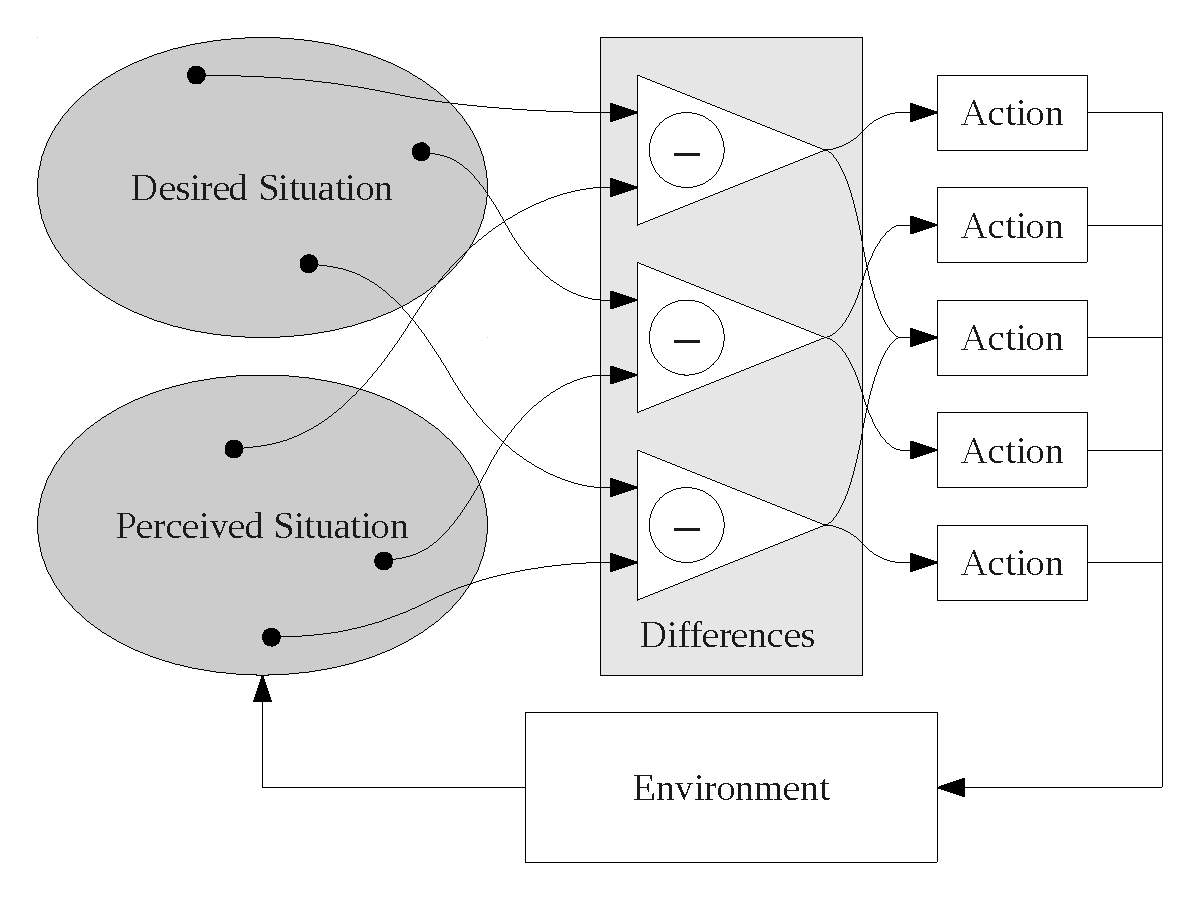
\includegraphics[height=6cm]{gfx/difference_engine_feedback_control}
  \caption[The difference engine model for accomplishing multiple goals]{The difference engine model for accomplishing multiple goals.}
  \label{fig:difference_engine_feedback_control}
\end{figure}

\citep[p.~78]{minsky:1988}



\section{Planning}

The real-time control aspect of my reflective control problem makes it
so that most planners and schedulers fail because they do not consider
their own run-time as a control problem, ad nauseam, which is my
proposed path around the general unconstrained logical reasoning
problem.  That said, there are a few modern advancements in combining
traditional planning techniques into larger learning systems that
confront the complexities introduced by acting in a domain.  Of these
planning or scheduling systems that are incorporated into systems that
act in domains, in which they have incomplete domain knowledge, there
are few systems that consider the real-time control aspects of not
only the domain, but the reasoning processes for acting in that domain
as well.

\subsection{Planning and Acting in Incomplete Domains}

\citep{weber:2011}


\subsection{Assuming a Correct Model of Environment}

There are many types of processes that make plans for accomplishing
goals, which make plans assuming a model of how actions theoretically
affect the environment.  These processes are called planners when they
create a representation for how actions should be performed,
potentially including temporal ordering constraints.

Planners are a specific part of a complete learning system, but the
primary function of a planner is to find a theoretical solution to a
given problem.  This theoretical solution, or plan, may be executed
and may fail or succeed, in accordance with the initial intentions for
executing the plan, the initial intentions for imagining the plan, or
any other intentions.  If the plan fails, then we may find something
to be modified in my knowledge in order to help us in avoiding this
failure next time.  The planning process is a small part of the
complete closed-loop learning algorithm that learns to plan from
experience with the environment and other AIs.



If we are thinking about the temporal constraints of the problem
solving process itself, then we need to consider a reflective approach
to this control problem.

  , (1) the model of the cause-effect relationship
between actions and the world, (2) the model of cause-effect
relationships between planning actions and the creation of successful
plans.

\subsection{Declarative Programming, Logical Reasoning}


\section{Machine Learning}

One encompassing goal of the field of machine learning is to develop
systems that can accomplish goals.

For example, a Markov Decision Process contains a transfer function,
which is basically a combinational device.

Of course, this combinational device would get complicated if I added probability.



\subsection{Why Did I Forget to Include Probability in my Theory?}



\subsection{The Reinforcement Learning Model}

\begin{figure}[bth]
  \center
  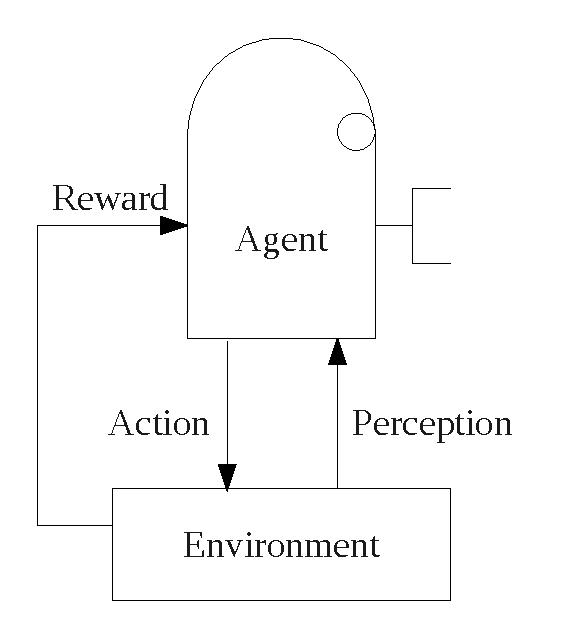
\includegraphics[height=5cm]{gfx/reinforcement_learning}
  \caption[The reinforcement learning model]{The reinforcement learning model.}
  \label{fig:reinforcement_learning}
\end{figure}

Figure~\ref{fig:reinforcement_learning} shows the basic reinforcement
learning model.  This model is an AI environment model, but there
is an extra information channel from the environment to the AI,
which communicates a numerical reward signal.  We can now say that the
AI has a learning problem.  The AI must learn what actions to
execute in order to gather the most reward.

\begin{figure}[bth]
  \center
  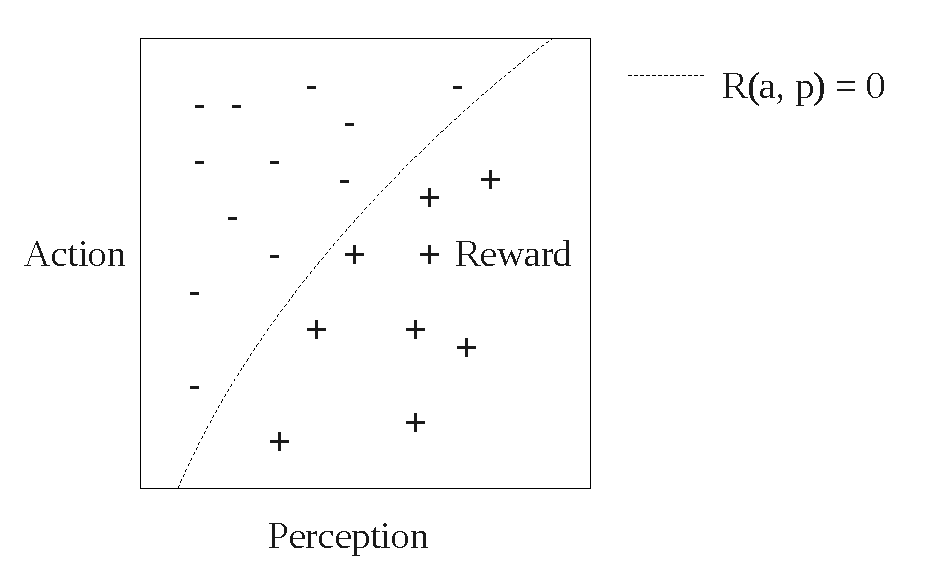
\includegraphics[height=4cm]{gfx/perception_categorization}
  \caption[Categorizing perceptions and actions based on goals]{Categorizing perceptions and actions based on goals.}
  \label{fig:perception_categorization}
\end{figure}

Once we have a basic reinforcement learning algorithm, we can approach
this learning problem as a function approximation problem.  In other
words, we can try to learn what parts of the perception and action
space have more or less reward.
Figure~\ref{fig:perception_categorization} shows a diagram of this
state space with the zero crossing of an approximation of the reward
plotted.

\subsection{Finding a Good Policy for Gathering Rewards}

Learning an approximation of what parts of a state space are good or
bad, based on reward, is not all that is needed to determine what
actions the AI should perform.  The AI wants to gather the most
rewards over time.  A simple way to formalize this problem is to learn
a policy that determines what action should be executed for every part
of the state space, based on some sort of summation of rewards over
time.  There have a been a number of ways of formalizing this
summation process as finite or infinite horizon problems
\citep{sutton:1998}.  Dynamic programming can be used for finding an
optimal or an approximately optimal policy \citep{bertsekas:1995}.

\subsection{Categorizing Perceptions and Actions based on Goals}

One problem with the reinforcement learning approach is that the only
representation of success or failure is a single number, the reward.
The basic reinforcement learning problem has been defined for finite
propositional state spaces.

A representation called \ac{RMDP} has been proposed
\citep{guestrin:2003} in order to extend reinforcement learning to
larger relational problem domains, but this method only focuses on an
object-oriented reward that does not have any global feedback about
the overall value of the situation.


\section{Philosophy}

\subsection{The Objective Modelling Assumption}

\begin{figure}[bth]
  \center
  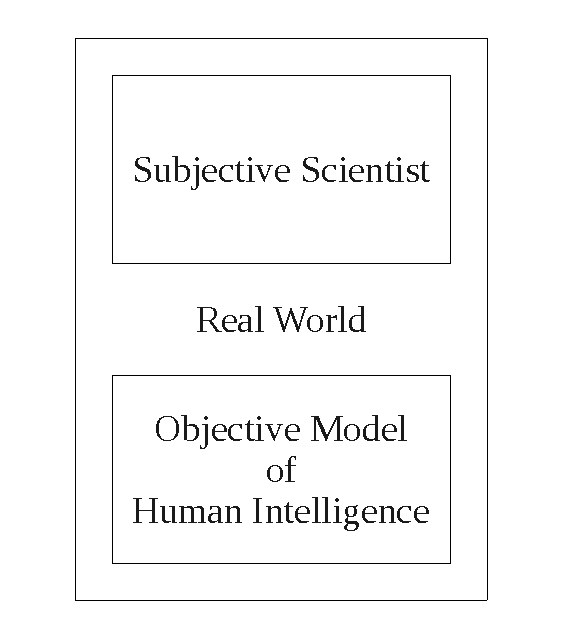
\includegraphics[width=4cm]{gfx/objective_description}
  \caption[The objective-subjective modelling assumption]{The objective-subjective modelling assumption.}
  \label{fig:objective_description}
\end{figure}

We assume that the phenomenon that we are trying to model, namely
human intelligence, is an objective process that we can describe.
This is the objective-subjective philosophical assumption that is
inherent in any objective scientific hypothesis.  We make this
assumption in order to avoid logical problems of circular causality
that occur when trying to find a non-objective description of
reflective thinking.  Figure~\ref{fig:objective_description} shows
how, given the objective assumption, the subjective scientist is part
of the real world, while she is studying an objective phenomenon.
Given the objective-subjective assumption, it would be a grave mistake
to confuse an objective model for reality itself.

\subsection{Being, Time, and the Verb-Gerund Relationship}

\subsection{The intensional stance}

\subsection{Reflective Representations}

\citep{perner:1991}


\section{Cognitive Science}


\subsection{The Development of Self-Conscious Emotions}

Between the ages of 1-3 years old, children display primary emotions,
such as joy, disappointment, and surprise.  These emotional processes
have been hypothesized to be related to the process of failing or
succeeding to accomplish a goal.  Around age 4, children begin to
display emotions that involve the self, such as guilt and shame.  It
has been hypothesized that these emotions relate to another person's
evaluation of the child's goals as good or bad.

We approach modelling this developmental process by applying Marvin
Minsky's theory of the child-imprimer relationship.  According to
Minsky's theory, at a young age, a human child becomes attached to a
person that functions as a teacher.  The imprimer could be a parent or
a caregiver or another person in the child's life, but the function of
the imprimer is to provide feedback to the child in terms of what
goals are good or bad for the child to pursue.

\subsection{Simulation Theory of Mind versus Theory Theory of Mind}


\subsection{Emotion or affect versus goal-oriented cognition}


\subsection{Embarrassment, Guilt, and Shame}



\section{Neuroscience}

\subsection{Neural Correlates of Consciousness}

\subsection{Learning by Positive and Negative Reinforcement}





\section{The Layered ``Model-6'' Theory for Organizing Reflective Models}

Because the many fields of human cognitive modelling are so disparate
it is difficult to see them as a whole.  I am inspired by a layered
organizational scheme first presented in \cite{minsky:2006}.  The
six layers in this ``Model-6'' organizational scheme are named as
follows:

\begin{enumerate}
\item{Instinctive Reactions}
\item{Learned Reactions}
\item{Deliberative Thinking}
\item{Reflective Thinking}
\item{Self-Reflective Thinking}
\item{Self-Conscious Reflection}
\end{enumerate}

I hope that the reader will see that this is a useful way of
organizing the massive amount of work that has gone into the
computational modelling of abstract human thought processes.

\subsection{Instinctive Reactions---Models of Insulation and Interaction}

\begin{quotation}
  \emph{We usually like to think in positive terms about how various parts of systems interact.}
  \emph{But to do that, we must first have good ideas about which aspects of a system do \emph{not} interact---since otherwise there would be too many possibilities to consider.}
  \emph{In other words, we have to understand \emph{insulations} before we can comprehend interactions.}
  \emph{To put this in a stronger form: \emph{No complicated society would actually work if it really depended on interactions among most of its parts}.}
  \emph{This is because any such system would be disabled by virtually any distortion, injury, or environmental fluctuation.}
  \emph{Nor could any such society evolve in the first place.}
\end{quotation}  

{\flushright{--- \cite{minsky:1988}}}

\subsubsection{Models of Failure in Distributed Systems}

\cite{attiya:2004} discuss algorithms for tolerating a few types of failures in distributed systems, ranging from silent crashes to arbitrary Byzantine failures, where parts of an algorithm perform in completely uncontrolled and unpredictable ways.
An algorithm for Byzantine tolerance is presented that is based upon building layers of first abstracting controllers that turn the Byzantine problem into a simpler \emph{identical Byzantine} problem.
The identical Byzantine problem is then abstracted to the simpler \emph{omission} problem, where a processor simply omits some messages from being transmitted.
The omission problem is then handled in a more abstract layer of the algorithm that when detecting an omission, crashes itself, resulting in a \emph{crash} problem.
Crash problems can be dealt in different ways for different algorithms, the simplest being the consensus algorithm.
This gives us a basic vocabulary of the most fundamental and basic distributed process problems.

\cite{bertsekas:1982} discuss a basic model for distributed dynamic programming that is organized around a distributed iterative approximation algorithm that computes a function mapping from states to values, $J(x){\in}\Re$.
His model divides the world into sets of states, $S_1 \cup S_2 \cup \cdots S_n = S$, that depend on neighboring sets of states in order to compute the approximation, $J^t$, of the optimal value function, $J^*$.
This fits with the idea that commonsense knowledge in an artificial intelligence program should be organized according to what goals it is important to solve.
Having a basic optimal control theory of why this is a fundamentally sound organization principle is encouraging: perhaps organizing our knowledge by the values of goal states could also apply in the context of abstract reinforcement learning.
Note that the information theoretic organizational approaches such as the inductive logic approach used by relational reinforcement learning do not organize their knowledge according to which goal values are important for calculating which other goal values.

\subsubsection{Models of Uncontrolled Distributed Statistical Inference}
Recently, statistical propositional logic has become popular along with graph-based inference techniques for calculating both the most likely propositional state as well as the probability of any single propositional variable.
Statistical models are often represented in graphical form that can be easily distributed and computed by sparse matrix multiplication algorithms.
Given a statistical model, it is common to use the MAXENT algorithm to approximate the most likely state of such a model.
\cite{jaynes:1982} discuss when this may or may not be appropriate.
\cite{murphy:1999} discuss Pearl's ``loopy'' belief propagation algorithm which is an unreliable but efficient inference tool.
\cite{yedidia:2005} generalizes this distributed form of statistical inference to hierarchical methods, explaining in the process that the forward-backward algorithm for hidden markov models, the Viterbi algorithm, Gallager's sum-product algorithm, the ``turbo-decoding'' algorithm, Pearl's ``belief propagation'' algorithm for inference on Bayesian networks, the ``Kalman filter'' for signal processing, and the ``transfer matrix'' approach in statistical mechanics are all of the same generalized form of statistical inference.

These statistical tools are the basic inference tools that claim nothing about their own applicability, and have no recourse for response for their own failures.
These statistical inference tools also know nothing about the goals which they are supposed to help solve.
In order for an algorithm to intelligently accomplish goals, it needs to deliberate or plan its usage of these most basic tools.

\subsubsection{Models of Distributed Intelligence}

\cite{maes:1990} discuss learning to coordinate behavior, an argument for robust robot control using multiple ways of reasoning in a layered architecture.

\subsubsection{Models of Computational Reflection}

\cite{maes:1987} gives a great overview of ``computational reflection,'' which is basically keeping track of information about the execution of a program, so that other processes can use that information to better control the program.
My approach to computational reflection is what they categorize as a ``frame-based'' approach, described first in \cite{minsky:1975} and first implemented in \cite{roberts:1977}.
\cite{maes:1987} describe the primary benefits of the frame-based approach as the following:

\begin{itemize}
\item{it helps the user cope with the complexity of a large system by providing documentation, history, and explanation facilities,}
\item{it keeps track of relations among representations, such as consistencies, dependencies and constraints,}
\item{it encapsulates the value of the data-item with a default-value, a form to compute it, etc.,}
\item{it guards the status and behavior of the data-item and activates procedures when specific events happen (e.g. the value becomes instantiated or changed).}
\end{itemize}

\cite{sobel:1996} discuss an introduction to reflection-oriented programming.
\cite{matsuoka:1992} discuss object-oriented concurrent reflective architectures.
\cite{oliva:1998} discuss the reflective architecture called ``Guaraná.''
\cite{watanabe:1989} discuss reflective computation in object-oriented concurrent systems.
\cite{yonezawa:1990} discuss a reflective object oriented concurrent language called ``ABCL/R.''
\cite{ancona:1998} discuss channel reification, which is a reflective model for distributed computation.
\cite{cazzola:1998} discuss evaluation of object-oriented reflective models.

\subsection{Learned Reactions---Models of Learning Reactions}

\subsubsection{Models of Planning to Perceive}

\cite{pryorcollins:1995} discuss how planning is used in perceptual processes.

\subsubsection{Models of Commonsense Reasoning}

There are many domains of quaitative commonsense reasoning, e.g. physics \cite[]{forbus:1994}, natural language \cite[]{liu:2004b}, story narratives \cite[]{williams:2005}, event planning \cite[]{smith:2006}, and psychology \cite[]{gordon:2008}.

\subsubsection{Models of Reactive Commonsense Knowledge}

There are also a few large knowledge bses of commonsense knowledge, e.g. ConceptNet \cite[]{liu:2004a}, FrameNet \cite[]{baker:1998}, Cyc \cite[]{lenat:1990}, AnalogySpace \cite[]{speer:2009}, and WordNet \cite[]{fellbaum:1998}.
Although these knowledge bases have a broad range of reasoning algorithms from linear algebraic semantic analogies in AnalogySpace to intricate microtheoretic logical deduction in Cyc, none of these knowledge bases are able to causal reflectively control the complexity of their algorithms.
Because commonsense knowledge is often represented in a declarative form, logical reasoning algorithms are often applied, but undirected logical reasoning methods often cannot handle large amounts of knowledge.
I see that reflective tools available in the Funk2 architecture could help with learning to reflectively control these explosive logical reasoning algorithms.

\subsection{Deliberative Thinking---Models of Learning to Compile Plans}

Planning and scheduling systems are useful for reasoning about, respectively: (1) what actions should be taken in a domain and (2) how those actions should be ordered in time \citep{smith:2000}.
\cite{michalski:1995} discuss learning as goal-driven inference.
\cite{weber:2011b} discuss counting failure explanations as a heuristic for guiding planning with knowledge seeking actions.
\cite{thagard:1995} discuss using a coherence theory of decision in order to perform inference to the best plan.

\subsubsection{Goal-Directed Knowledge Acquisition}

\cite{weber:2011b}

\subsubsection{Reinforcement Learning}

According to \cite{sutton:1998}, the field of reinforcement learning deals with the problem of ``learning what to do---how to map situations to actions---so as to maximize a numerical reward signal.''
Reinforcement learning is an online type of learning problem as opposed to supervised or unsupervised types of learning problems.

\cite{kaelbling:1996} gives a good overview of historical reinforcement learning.
The reinforcement learning problem is defined as

\begin{itemize}
\item{a set of states, $\mathcal{S}$,}
\item{a set of actions, $\mathcal{A}$, and}
\item{a set of scalar reinforcement signals, typically $\{0,1\}$ or $\Re$.}
\end{itemize}

It is interesting to consider how the well developed idea of ``exploration versus exploitation'' as discussed in \cite{kaelbling:1996} as a model for deciding when to sequentially meta-reason.

subsubsection{Models of Optimal Behavior}

\cite{kaelbling:1996} discuss three primary models of optimal behavior:

\begin{enumerate}
\item{the \emph{finite horizon} model in which an AI performs receding horizon control, such that total reward is $E(\sum_{t=0}^{h}{r_t})$,}
\item{the \emph{infinite discounted} model in which an AI uses future rewards discounted by a constant factor, $\gamma$, such that total reward is $E(\sum_{t=0}^{\infty}{\gamma^t r_t})$, and}
\item{the \emph{average reward} model which is the infinite limit of the finite horizon model, such that total reward is $\lim_{h{\rightarrow}\infty}{E(\frac{1}{h}\sum_{t=0}^{h}{r_t})}$.}
\end{enumerate}

These exact optimality criteria are only applicable to relatively small problem domains.
Nonetheless, I hypothesize that useful approximations of optimal systems that can be derived from overlapping subsystems with constraining optimality criteria can be derived from these three basic types of optimality.
Homeostasis monitors and continual ``heartbeat'' controllers could be implemented with infinite or average optimality models, while short-term goal-oriented controllers would necessitate the complexities of the full $N$-step finite horizon model of optimality.

\subsubsection{Dynamic Programming and Optimal Control}

\cite{bertsekas:1995} describe techniques for finding optimal and approximate \emph{functional} (\emph{memoizable}) solutions to reinforcement learning control problems, using recursive formulas of flat state spaces that can be optimized very easily by using memoized functions.
While this approach does not handle abstract models of the AI's world, there are exciting options of combining a dynamic programming approach with an abstract form of reinforcement learning, such as the use of inductive logic described in \cite{dvzeroski:2001}.

\subsubsection{A Theoretical World Model}

A simple formulation of the reinforcement learning problem can be formulated in terms of Markov Decision Process (MDP) environments.
An MDP is defined as

\begin{itemize}
\item{a set of states, $\mathcal{S}$,}
\item{a set of actions, $\mathcal{A}$,}
\item{a reward function $\mathcal{R}:\mathcal{S}\times\mathcal{A}\rightarrow\Re$, and}
\item{a state transition function, $\mathcal{T}:\mathcal{S}\times\mathcal{A}\rightarrow\Pi{(\mathcal{S})}$.}
\end{itemize}

\subsubsection{Category Learning to Accomplish Goals}

Category learning in the context of goal-oriented problem-solving is an idea that is discussed by \cite{barsalou:1995}.

\subsubsection{Models of Learning by Positive or Negative Reward in the context of Relational Knowledge}

\cite{dvzeroski:2001} describe an interesting combination of inductive logic programming (ILP) \cite[]{muggleton:1992} and reinforcement learning.
The benefit of using abstract logical representations of propositional states, actions, and state values makes the basic reinforcement learning algorithm able to deal with relational state spaces, such as the blocks world toy problem and the other problem representations that I am focusing on in this PhD.
This form of learning abstractions takes a flat mental space and maps it to a hierarchical relational abstraction.

\subsection{Reflective Thinking---Models of Learning to Control Deliberation}

\subsubsection{Models of Commonsense Psychology}

Understanding human psychology in commonsense terms is an initiative described in \cite{gordon:2004}.
I see my work as building upon this development of a commonsense language for discussing the types of mental processes that humans have.
Also, \cite{gordon:2008} further develops this commonsense psychological language approach to describe the processes of self-reflection, which is relevant to my work.
The difference between my approach and the commonsense psychology approach is that my work simulates these mental processes in a computer, using the Funk2 causally reflective procedural programming language.
Previous approaches have represented psychological reasoning processes in a declarative logical form, but these logical forms cannot handle the large knowledge bases that are involved in general commonsense reasoning.

\cite{wilson:1977} discuss verbal reports on mental processes.
\cite{schank:1972} discuss primitive concepts underlying verbs of thought.

\subsubsection{Models of Unsticking Deliberation by Creative Analogical Thinking}

\cite{buchanan:1977} discuss creativity at the metalevel.
\cite{mueller:1990} discuss daydreamer.

A storytelling system that is called MINSTREL is discussed in \cite{turner:1994}; it is guided by creativity goals in order to develop good narratives.
The process of creative storytelling is handled very similarly to mechanical goal-oriented problem solving in this way.

\subsubsection{Models of Learning to Plan to Learn}

\cite{ram:1995a} discuss planning to learn.
\cite{desjardins:1995} discuss a decision-theoretic model for deciding what to learn next for accomplishing goals.
\cite{ram:1995b} discuss goal-driven learning in multistrategy reasoning and learning systems.
\cite{ram:1995c} discuss learning, goals, and learning goals.
\cite{cox:1999a} discuss the construction of learning strategies in introspective multistrategy learning.

\subsubsection{Models of Learning by Credit Assignment through Temporal State Tracing}

\emph{Eligibility traces} are a simple reinforcement learning tool for temporal credit assignment for an AI entering positive and negative reward states.
For example, the \emph{backward} view of eligibility tracing as applied to the temporal difference, $\text{TD}(\lambda)$, learning method simply augments the basic learning algorithm with an additional eligibitity factor, $e_t(s)$, for each state.
Only non-zero values of the eligibility factor are remembered in tractible (approximate) implementations; this amounts to keeping a list of $n$ recently visited states.
In the algorithm, the current state's eligibility factor, $e_t(s_t)$, is set to $1$ and all other states are discounted by a constant eligibility discount factor, $\gamma$.
Credit assignment for rewards that are found in the world are assigned not only to the previous state, as in the basic one-step $\text{TD}(\lambda)$ algorithm but also assigned to the value functions in a discounted sense to the previous $n$ states in its eligibility trace.
I call this form of credit assignment ``Temporal State Tracing'' because it simply assigns credit to those states temporally local to the current state, i.e. there is no explicit consideration of causality involved in the assignment.

\subsubsection{Models of Learning by Credit Assignment through Causal Tracing of Failure}

I do not know of any reinforcement learning algorithms that reflectively learns how to plan through causal tracing of failures.
My method of learning in this way is disussed in Section~\ref{causal_tracing_of_failure-section}.

\subsubsection{Models of Learning by Explaining Failures}

\cite{hammond:1990} discuss explaining and repairing plans that fail.
\cite{vanlehn:1992} discuss a model of the self-explanation effect.
\cite{ram:1995d} discuss introspective reasoning using meta-explanations for multistrategy learning.
\cite{leake:1995a} discuss goal-based explanation evaluation.
\cite{leake:1995b} discuss toward goal-driven integration of explanation and action.
\cite{dominowski:1998} discuss verbalization and problem solving.

\subsubsection{Models of Learning by Repairing Failed Plans and Inference Knowledge}

\cite{leake:1996} discuss learning to refine the case-based reasoning process through experience, introspection and expertise.
\cite{levin:2004} discuss how to span the difference between metacognitive failure and success in thinking about seeing.
\cite{cox:1996} discuss how to construct a learning strategy under reasoning failure in the terms of introspective multistrategy learning.

\subsubsection{The Difference between Metareasoning, Computational Reflection, and Causal Reflection}

\cite{hansen:2001} discuss a dynamic programming approach to monitoring and control of anytime algorithms.
\cite{cox:2007a} discuss metareasoning, monitoring, and self-explanation.
\cite{cox:2005} present a selected research review of metacognition in computation.
\cite{anderson:2007} present a review of recent research in metareasoning and metalearning.
\cite{cox:2007b} discuss perpetual self-aware cognitive AIs.
\cite{cox:2008} present a manifesto on metareasoning.
\cite{davis:1980} discuss reasoning about control in terms of meta-rules.
\cite{fox:2001} discuss introspective reasoning for index refinement in case-based reasoning.
\cite{maes:1988} discuss issues in computational reflection.
\cite{minsky:1968} discuss matter, mind, and models.
\cite{newell:1982} discuss the knowledge level.

\subsubsection{Empirical Models of Reflective Thought}


\cite{baumeister:2007} discuss How emotion shapes behavior: Feedback, anticipation, and reflection, rather than direct causation.
\cite{vince:2002} discuss Organizing reflection.
\cite{mirvis:2008} discuss Executive Development Through Consciousness-Raising Experiences.
\cite{michalsky:2007} discuss Developing Students' Metacognitive Awareness in Asynchronous Learning Networks in Comparison to Face-to-Face Discussion Groups.
\cite{bivona:2008} discuss Executive function and metacognitive self-awareness after Severe Traumatic Brain Injury.
\cite{irannejad:2001} discuss The brain-mind cycle of reflection.
\cite{phillips:2005} discuss Self-awareness and the emotional consequences of self-discrepancies.
\cite{silvia:2006} discuss Emotion concepts and self-focused attention: Exploring parallel effects of emotional states and emotional knowledge.
\cite{lynn:2008} discuss The eq interview: finding employees with high emotional intelligence.


\subsection{Self-Reflective Thinking---Models of Control using Self and Other Models}

\cite{anderson:2005} discuss the metacognitive loop and the problem of brittleness in terms of logic, self-awareness and self-improvement.
\cite{schubert:2005} discuss some knowledge representation and reasoning requirements for self-awareness.

\subsubsection{Models Involving Multiple AIs}

Models of multiple intelligent AIs that work together to solve problems have become popular in the field of machine learning called ``multi-AI reinforcement learning.''
Many popular surveys of the field exist \cite[]{wei:1995} \cite[]{sen:1999} \cite[]{stone:2000} \cite[]{shoham:2004} \cite[]{yang:2004} \cite[]{panait:2005}.

\cite{boutilier:1996} discuss a specific type of $n$-person cooperative game theory, in which AIs share common goals, or in other words, a joint value function.
\cite{rapoport:2001} discuss $n$-person game theory in detail.

\cite{bowling:2000} describe an analysis of stochastic game theory for multiAI reinforcement learning.
\cite{claus:1998} describe the dynamics of reinforcement learning in cooperative multiAI systems.
\cite{crites:1998} describe elevator group control using multiple reinforcement learning AIs.
\cite{ghavamzadeh:2006} describe hierarchical multi-AI reinforcement learning.
\cite{guestrin:2002} describe coordinated reinforcement learning.
\cite{hu:1998} describe a theoretical framework and an algorithm for multiAI reinforcement learning.
\cite{kapetanakis:2002} describe reinforcement learning of coordination in cooperative multi-AI systems.
\cite{mataric:1997a} describe reinforcement learning in the multi-robot domain.
\cite{park:2001} describe modular $Q$-learning based multi-AI cooperation for robot soccer.
\cite{sandholm:1996} describe multiAI reinforcement learning in the iterated prisoner's dilemma.
\cite{tan:1997} describe independent versus cooperative AIs in multi-AI reinforcement learning.
\cite{wang:2003} describe reinforcement learning to play an optimal Nash equilibrium in team Markov games.

\subsubsection{MultiAI Reinforcement Learning with Layered Models}
\cite{stone:1997} describe layered Learning in multiAI Systems.

\subsubsection{MultiAI Reinforcement Learning with Communication}

\cite{drogoul:1994} describe an application to social differentiation in ant colonies using a multi-AI simulation as a tool for modeling societies.
\cite{fischer:2004} describe hierarchical reinforcement learning in communication-mediated multiAI coordination.
\cite{price:1999} describe implicit imitation in multiAI reinforcement learning.
\cite{sen:1998} describe individual learning of coordination knowledge.

\subsubsection{MultiAI Reinforcement Learning with Self- and Other- Models}

\cite{mataric:1997b} describe learning social behavior.
\cite{nagayuki:2000} describe an approach based on the otherAI's internal model in multi-AI reinforcement learning.
\cite{noble:2004} describe social learning in a multi-AI system.
\cite{nowe:2001} describe social AIs playing a periodical policy.

\subsubsection{Models of Parent and Child Social Functions}
\cite{castelfranchi:2001} describe the challenges for computational social science and multi-AI learning in a theory of social functions.


\subsubsection{Empirical Models of Inferring Person Traits}

\cite{asch:2005} discuss how impressions of personalities are formed.
They break personality down into $18$ two-part models, or dimensions.
See Table~\ref{tab:asch_personality_dimensions} for a listing of these dimensions.

\begin{table}
  \myfloatalign
  \begin{tabularx}{\textwidth}{XlllX}
    & 1.         & generous           & ungenerous    & \\
    & 2.         & wise               & shrewd        & \\
    & 3.         & happy              & unhappy       & \\
    & 4.         & good-natured       & irritable     & \\
    & 5.         & humorous           & humorless     & \\
    & 6.         & sociable           & unsociable    & \\
    & 7.         & popular            & unpopular     & \\
    & 8.         & reliable           & unreliable    & \\
    & 9.         & important          & insignificant & \\
    & 10.        & humane             & ruthless      & \\
    & 11.        & good-looking       & unattractive  & \\
    & 12.        & persistent         & unstable      & \\
    & 13.        & serious            & frivolous     & \\
    & 14.        & restrained         & talkative     & \\
    & 15.        & altruistic         & self-centered & \\
    & 16.        & imaginative        & hard-headed   & \\
    & 17.        & strong             & weak          & \\
    & 18.        & honest             & dishonest     & \\
    & \emph{19.} & \emph{warm}        & \emph{cold}   & \\
    & \emph{20.} & \emph{intelligent} & ~             & \\
    & \emph{21.} & \emph{envious}     & ~             & 
  \end{tabularx}
  \caption[18 personality dimensions]{18 personality dimensions discussed by \cauthor{asch:2005}.}
  \label{tab:asch_personality_dimensions}
\end{table}


\cite{winter:2005} discuss the difference between \emph{dispositional} inferences and \emph{situational} inferences.
A dispositional statement is a statement about the relationship between person models, such as ``kind person'' or ``she helped the man'', whereas a situational statement is a statement that does not refer to such a model of a social relationship between person models, such as ``she dropped the groceries''.
See Table~\ref{tab:winter_dispositional_properties} for the list of 18 dispositional properties that they discovered in their research interviewing college students for word associations:

\begin{table}
  \myfloatalign
  \begin{tabularx}{\textwidth}{XllX}
    & 1.  & generous          & \\
    & 2.  & rude              & \\
    & 3.  & good worker       & \\
    & 4.  & helpful           & \\
    & 5.  & ill-mannered      & \\
    & 6.  & thrifty           & \\
    & 7.  & talented          & \\
    & 8.  & bigot             & \\
    & 9.  & friendly          & \\
    & 10. & concerned citizen & \\
    & 11. & absent-minded     & \\
    & 12. & kindhearted       & \\
    & 13. & cheap             & \\
    & 14. & clever            & \\
    & 15. & inconsiderate     & \\
    & 16. & willpower         & \\
    & 17. & considerate       & \\
    & 18. & clumsy            & 
  \end{tabularx}
  \caption[18 dispositional properties]{18 dispositional properties
    that \cauthor{winter:2005} discovered in their research
    interviewing college students for word associations.}
  \label{tab:winter_dispositional_properties}
\end{table}


\subsubsection{Empirical Models of Self and Other Social Models}

This section discusses much research that often uses words that I often do not see used precisely.
For example, the phrase ``self-awareness'' is often used to describe a sort of mental process that monitors another mental process.
In this document, I try to be consistent by using the word ``self'' to only refer to models of self versus other in terms of AIs thinking about personalities or properties of AIs.
Other common uses of the terms ``self-awareness'' and ``self-consciousness'' are often less clear and refer to any kind of reflective process perceiving the execution of another process within the mind.
There are many forms of reflective thought, and I choose to use the term ``self-reflection'' to refer to those reflective processes that deal with self and other personality models of inter-AI relationships.

\cite{goverover:2007} discuss treatment to improve self-awareness in persons with acquired brain injury.
\cite{baumeister:1993} discuss when ego threats lead to self-regulation failure: negative consequences of high self-esteem.
\cite{gilbert:2005} discuss perceptions of people.
\cite{ross:2005} discuss social roles, social control, and biases in social-perception processes.
\cite{hobson:2006} discuss self-awareness in developmental perspective.
\cite{hutchinson:2007} discuss relationships among adaption-innovation, self-monitoring, and self-consciousness.
\cite{keenan:2007} discuss the selective causal role of the right hemisphere in self-awareness.
\cite{morin:2004} discuss a comparison and integration of various views of the levels of consciousness and self-awareness.
\cite{silverman:2008} discuss self-reflection.
\cite{smith:2007} discuss self-awareness, perspective-taking, and self-face recognition.
\cite{soeiro:2008} discuss state versus trait self-focus: comparing self-awareness to self-consciousness.
\cite{uhlmann:2008} discuss varieties of social cognition.
\cite{burns:1998} discuss individual selves, self-awareness, and reflectivity in the social construction of consciousness.
\cite{duval:2002} discuss self-awareness, probability of improvement, and the self-serving bias.
\cite{focquaert:2008} discuss an evolutionary cognitive neuroscience perspective on human self-awareness and theory of mind.
\cite{whitehead:2001} discuss social mirrors and shared experiential worlds.


\subsubsection{Empirical Models of Person Groups}

\cite{menon:2005} discuss the attribution to individual versus group dispositions in culture and the construal of agency.

\subsection{Self-Conscious Reflection---Models of Learning by Imprimer Reflection on Self and Other Models}

\subsubsection{Empirical Models of Imprimers}

\cite{hinton:2008} discuss the role of leader self-awareness in building trust and improving student learning.
\cite{taylor:2007} discuss a conceptual framework and an empirical test for determining leader attunement in order to work toward developing a more general theory of leader self-awareness.
\cite{hare:1993} describe how certain types of anti-social personality disorders result in ``successful'' individuals and a disturbing view of society.

\subsubsection{Moral Decisions and Values}

\cite{harsanyi:1980} discuss rule utilitarianism, rights, obligations and the theory of rational behavior.
\cite{duval:1999} discuss how changing self or changing standards of correctness also changes objective self-awareness and causal attributions for self-standard discrepancies.


\section{Natural Language in Problem-Solving}

\cite{bobrow:1968} discuss a system that processes natural language in
the context of automated problem-solving.



\section{Models of Story and Language Understanding}


\cite{ram:1999a} present a theory of reading and understanding.
\cite{ram:1999b} present a theory of questions and question asking.
\cite{rapaport:1999} discuss automated language understanding in fiction.
\cite{mahesh:1999} discuss sentence processing while integrating multiple knowledge sources.
\cite{domeshek:1999} discuss parsing the semantic content from complex narratives.
\cite{peterson:1999} discuss a theory of semantic correspondence.
\cite{moorman:1999} discuss learning novel concepts requiring creativity while reading.
\cite{cox:1999b} discuss the intersection of story understanding and machine learning.
\cite{gerrig:1999} discuss natural language text processing in narrative worlds.

\section{Evaluating Models of Complex Learning}


\subsection{Evaluating Models of Learning Skill Knowledge}
\cite{anderson:1993} describe subjects acquisition of LISP programming skills in an experimental setting.
\cite{ohlsson:1993} describe the acquisition of cognitive skills while fosucing on the interaction between knowledge and practice.

\subsection{Evaluating Models of Learning by Self-Explanation}
\cite{vanlehn:1993} present a computational model of the process of learning by explaining examples to oneself.
\cite{kieras:1993} describe a model of learning schemas from explanations in the domain of practical electronics.
\cite{rosenbloom:1993} discuss the problem of learning bias in planning and explanation-based learning.

\subsection{Evaluating Models of Learning Declarative Relational Knowledge}
\cite{huffman:1993} analyze the knowledge-level of a model that corrects imperfect domain theories.
\cite{hammond:1993} present a cognitive science approach to case-based planning.
\cite{wilensky:1993} discuss the problem of knowledge acquisition in the domain of natural language processing.

\subsection{Visual Programming Languages for Psycological Study of Complex Models}

\cite{cooper:2002} and \cite{cooper:1998a} discuss how to model high-level cognitive processes in an empirical and scientific way.
Much of their work is presented in terms of their COGENT cognitive architecture that includes a visual programming language for cognitive scientists to quickly build and evaluate varieties of complex hypotheses.

\cite{cooper:1995} discuss an object-oriented language for cognitive modeling.
\cite{cooper:1996} discuss a systematic methodology for cognitive modelling.
\cite{cooper:1998b} discuss their system, COGENT, an tool for the development of cognitive models.
\cite{councill:2003} analyze existing tools and user information requirements with regard to the Soar cognitive architecture.
\cite{mulholland:1998} discuss their Hank system, a friendly cognitive modelling language for psychology students.
\cite{mulholland:1999} discuss how the Hank system can be used for implementing schema theory.
\cite{mulholland:2000} discuss an educational tool for psychology students to learn by building computational cognitive models.
\cite{yule:2001} discuss a vision of a technology for efficienct experimentation with computational cognitive models.

\section{Models of the Large-scale Integration of Multiple Models of Cognition}

\cite{langley:2008} gives a good overview of the current state of the field of cognitive architectural design in terms of what exists and what needs to still be designed and built.
Among the features that are not much explored are the types reflective processes that control deliberative processes, which \cite{sloman:2001} refers to as meta-management.
I see building layers of these reflective management processes in the top three layers of the Emotion Machine theory as my basic inspiration for higher orders of reflective control beyond meta-management.

\subsection{The EM-ONE Model}

\cite{singh:2005} describe the first cognitive architecture based on the Emotion Machine theory of mind, developed in \cite{minsky:2006}.
This architecture includes the ability to control reasoning using a relational list commonsense narrative representation.
In terms of types of representations, the Emotion Machine theory proposes that self models exist in the self-reflective layer and imprimer models exist in the self-conscious layer.
My purpose is to elaborate on this example model in a larger and causally reflective programming language.
My Funk2 architecture is based on procedural forms of run-time reflection that is built into the underlying programming language, whereas the previous work was based on declarative forms that used an assortment of programming languages, including Lisp and Prolog.

\subsection{The Icarus Model}

\cite{langley:2005} describe an architecture that uses meta-knowledge of knowledge.
They refer to skill planning as planning toward long-term goals in the abstract meta-knowledge plan space.
They refer to short-term planning as planning over instances of the skill plans.
I see my approach as complimentary to this plan abstraction approach because I am focused on adaptive learning due to failures of conflicting plans, so I expect my approach to be adaptable to this form of meta-planning as well.

\subsection{The ACT-r Model}

\cite{anderson:2004} describe a model that is inspiring to us because it is the largest cognitive architecture that is actively being correlated to human neurological and psychological data.
I see my work as heading in this direction, but first I must complete a working model of my theory so that such similar scientific work may proceed in terms of understanding reflective, self-reflective, and self-conscious thought processes.

\subsection{The SOAR Model}

\cite{laird:1987} describe the SOAR cognitive architecture, an architecture for general intelligence.
\cite{marinier:2009} describe a recent use of SOAR to build a model that unifies cognitive behavior and emotion.

\subsection{The PolyScheme Model}

\cite{cassimatis:2004} and \cite{cassimatis:2006} describe a cognitive architecture that combines multiple representations and reasoning methods for implementing human level intelligence.
I see the problem of having multiple representations and concurrent reasoning processes as exactly the problem that I am designing the Funk2 causally reflective architecture: in order to control and learn from conflicts in such a mental model.

\subsection{The GLAIR Model}

\cite{shapiro:2003} describe an architecture that performs a form of belief revision.

\subsection{The CIRCA Model}

\cite{musliner:2001} describe an architecture with plan execution processes that operate in real-time concurrently with deliberative planning processes.
This architecture is not reflective over it's deliberation, but Funk2 is designed with this concurrency and real-time behavior in mind as well.

\subsection{The CogAff Model}

\cite{sloman:2001} describe a three-layer cognitive architecture that is very similar to the bottom three layers of the Emotion Machine theory's bottom three layers, i.e. reactive, deliberative, and meta-management or reflective layers.
The CogAff architecture does not make any representational commitments and higher layers of reflection are referred to as complex forms of meta-management.

\subsection{The Three Layers Model}

\cite{ngbereiter:1995} discuss three levels of goal orientation in learning.

\subsection{The AIS Model}

In \cite{hayesroth:1995}, a reflective architecture is described that operates on cycles.
On each cycle, a meta-cognitive controller selects among a set of deliberative controllers.

\subsection{The Prodigy Model}

\cite{carbonell:1991} describe an architecture that learns to plan through self-explanation and using what they refer to as causal traces of execution histories.
These causal traces are similar to what can be derived from the causal tracing functionality inherent in the Funk2 programming language.

\cite{carbonell:1995} discuss planning and learning in PRODIGY, an integrated architecture.

\subsection{The Daydreamer Model}

\cite{mueller:1990} describes a model containing a ``society of mind''
collection of deliberative thinking resources that perform many
different types of planning and analogical transfer between different
mental realms.



\section{Parallel-Lisp Programming Languages}

\cite{halstead:1990} discusses parallel lisp language design, implementations, and programming tools.


















































